\documentclass[a4paper,11pt]{report}
\usepackage[T1]{fontenc}
\usepackage[utf8]{inputenc}
\usepackage[italian,english]{babel}
\usepackage[margin=2.5cm]{geometry}

\usepackage{graphicx} % Required for inserting images
\usepackage{makeidx}
\usepackage{float}
\usepackage{chngcntr}
\usepackage{minted}
\usepackage{listings}
\usepackage{hyperref}
\hypersetup{%
    pdfpagemode={UseOutlines},
    bookmarksopen,
    pdfstartview={FitH},
    colorlinks,
    linkcolor={blue},
    citecolor={blue},
    urlcolor={blue}
}


\usepackage{parskip} % Aggiungi il pacchetto per la gestione degli spazi tra i paragrafi
\setlength{\parindent}{0pt} % Imposta lo spazio tra i paragrafi a 0pt
%\usepackage{titlesec}
%\titlespacing{\section}{0pt}{5ex}{2ex}
%\titlespacing{\subsection}{0pt}{5ex}{2ex}

\counterwithout{section}{chapter} % Rimuove il numero del capitolo dalla numerazione delle sezioni
\setcounter{section}{0} % Imposta la numerazione delle sezioni a partire da 1


\begin{document}

    %%INTESTAZIONE
	\begin{titlepage}
		\begin{center}
            \vspace*{-3cm}
	
		\includegraphics[width=0.72\textwidth]{logo}~\\[0.8cm]
		
		\textsc{\LARGE Politecnico di Torino}\\[0.5cm]
		
		\Large Master's Degree in Computer Engineering\\
        \Large Cybersecuirty\\[0.1cm]
        \vspace*{1.2cm}
	
		\textsc{\Large Computer Architectures and Operating Systems}\\[0.8cm]
        \large A.Y. 2023/2024\\[0.1cm]
		\vspace*{1.5cm}
			
		% Title
		{ \LARGE \bfseries Report BoardOS project\\[2.5cm] }

        % Authors
		\noindent
		\begin{minipage}[t]{0.9\textwidth}
			\begin{flushright} \large
				\emph{\textbf{Authors and student IDs:}}\\
	            Jacopo \textsc{Coniglio} - 328770\\
                Francesca \textsc{Coriale} - 330700\\
                Sibilla \textsc{Merlo} - 319248\\
                Giulia Lydia \textsc{Perini} - 280891\\
                Ankesh \textsc{Porwal} - 328746\\
			\end{flushright}
		\end{minipage}
        \end{center}
    \end{titlepage}


    %%blank page
    %%\thispagestyle{empty}
    %%\mbox{}
    %%\newpage
    
    %%index
    \addtocounter{page}{-1} %%levare numero zero da indice 
	\tableofcontents
    \thispagestyle{empty}
	\newpage


%%\chapter{}
\section{Objectives}
The aim of the project is to acquire proficiency in the usage of an embedded system on an ST Nucleo Board, specifically STM32 Nucleo-64 Board, paired with a STM32F446RE microcontroller.

The project is articulated into four distinct points:
\begin{enumerate}
    \item developing a tutorial detailing the installation and usage procedures;
    \item defining practical exercises illustrating the functionalities of the board;
    \item showing a customization of the operating system;
    \item comparing evaluations and benchmarks of the performances achieved by the newly implemented solution.
\end{enumerate}

The focus of the report will be on providing an outline of the project execution. For further and detailed information, please refer to the material uploaded on GitLab.

The tutorial is accessible at the following \href{https://baltig.polito.it/caos2023/group2/-/blob/point1/point1.md}{page}.

\section{Overview}
For the development of this project we used a STM32 Nucleo 64 Board. \\
Some characteristic of the board are: 
\begin{itemize}
\item three LEDs:  USB communication (LD1), user LED (LD2), power LED (LD3);
\item two push-buttons: \texttt{USER} (also referred to it as "Blue Button" in this report) and \texttt{RESET};
\item on-board ST-LINK/V2-1 debugger;
\item virtual COM port (in our case used for UART transmission).
\end{itemize}
We decided to use FreeRTOS as main operating system. 
For the exercises in point 2 we have always included CMSIS-V1, since it offers a common API standard for ARM Cortex-M microcontrollers, such as the one on the Nucleo.  \\
As developement environment we chose STMCubeIDE, being the most recommended by STM32 itself.\\ 
For printf debugging we used the SWV window inside STMCubeIDE or a serial port terminal (Hercules) to catch the data transmitted via the UART.

\section{Exercises}
\subsection{Scheduling of FreeRTOS}
The first example we developed is to show how the default scheduling of FreeRTOS works: we have a preemptive scheduling based on priority, hence higher priority tasks, when ready, can preempt lower priority tasks. \\
After the operation \texttt{osKernelStart()} in the main function, the control is given to the scheduler and the scheduling algorithm. 
In the specific example developed we have three tasks: high, medium and low priority. The first task chosen by the scheduler is the high priority task, which is executed 3 times before ending  with \texttt{osTaskExit()}.\\
Then it will be the turn for the medium task and subsequently for the low task, and both will do the same thing as the high priority task.

\subsection{LCD}
In this example we experiment a little with external peripherals that can be connected to the board. We decided to wire a LCD1602 to the board, linking the 16 pins of the display (retroillumination, power, gdr, data communication, etc.) to the board. \\
The Nucleo-F446RE board for the GPIO pins has ports from A to K with 16 pins each. \\
We also include the \texttt{lcd.c} code that implements specific functions for the functioning of the LCD, such as initialization and displaying of characters. This kind of display has 2 rows of 16 columns each. \\
The code implements a 10 minute timer (the time given for our presentation) and generates a string to display the "Time left" on the LCD display.
   
\subsection{LED blink with Interrupt}
In this example it is shown how to update the status of the green LED using the Blue Button. More in detail, we want that every time the Blue Button is pressed the LED changes its status. To do so we link the status of the LED to the value of a counter, which is incremented by 1 with the pressing of the Blue Button.\\
The different LED patterns are:
\begin{itemize}
    \item if the \texttt{counter = 0}, then it blinks with a period of $0.5$ seconds;
    \item if the \texttt{counter = 1}, then it remains lit;
    \item if the \texttt{counter = 2}, then it remains off;
\end{itemize}
if the \texttt{counter = 3}, we start again the cycle by setting the counter equal to zero.\\
Since we can press the button at any time, we require that every time the button is pressed, any running task is stopped and the counter is updated. This type of command is performed by an Interrupt, triggered by the pressing of the button. This can be done by setting the Blue Button as trigger for the interruption in the configuration window.\\
In the \texttt{main.c} file then we have to declare and define the default task in charge of controlling the LED based on the value of a counter and the callback function, that will be automatically called when the external interrupt (\texttt{EXTI}) occurs on the GPIO PIN associated to the Blue Button and will update the counter.\\
After the interruption, the default task will select the correct status for the LED based on the value of the counter.
  
\subsection{Priority Inversion}
This is an ad-hoc example to show how priority inversion can happen in real-time systems based on preemption. This can happen for example when a low priority task is holding a lock that an high priority task needs to continue its execution.\\
In general, we can have two types of priority inversion: \textit{bounded} or \textit{unbounded}. In this instance we are looking at the unbounded one: an high priority task is blocked by a low priority task, that is also waiting for a medium priority task to finish. So, the medium task can now effectively block the high task for any amount of time, since medium task is preempting the low task. \\

\begin{figure}[H]
    \centering
    \includegraphics[height=6.5cm]{unbounded_priority_inversion.jpg}
\end{figure}

In the example developed we have three tasks: H (high priority), M (medium priority) and L (low priority). \\
H and L uses a binary semaphore to enter in what we can call the \textit{critical section}: a snippet of code that must be executed atomically. L, once entered in the critical section, waits for the Blue Button on the board to release the before-acquired semaphore. H acquires the semaphore, writes a message and then releases it. M has an independent execution, in which it prints a message and then ends.\\
What happens is that, after L acquires the semaphore it has to wait for the user to push the button in order to release the lock: H is then blocked since it can't acquire the semaphore, and L, even if the button is pressed, is preempted by M. \\
One of the possible solutions to priority inversion is \textit{priority inheritance}. Priority inheritance consists in boosting the priority of a task holding a lock to that of any another higher priority task that tries to take the lock. In this way a higher priority task cannot be preempted by a lower priority task holding the required lock.
FreeRTOS and CMSIS-RTOS provide a mechanism for priority inheritance, implemented with mutexes. \\
Whenever a lower priority task acquires and holds a mutex, its priority is temporarily raised to the priority of the highest-priority task that is waiting for the same mutex. Note that, after the mutex has been released, the priority of the task is restored to the original value.\\
In this exercise we implemented the previous example with mutexes instead of binary semaphores. Now, whenever the low priority task takes the mutex, the medium task is not able to preempt it, since the priority of the low task is raised to the one of the high task. \\


\section{Customization of the OS and benchmarks}
In this final part of the project we want to modify some of the functions in the Kernel of the operating system FreeRTOS and benchmark the performance improvement achieved by the newly implemented solution.
\subsection{Tasks scheduling}
We analyzed a particular behaviour that occurs in a program when we have three tasks with different priorities (this can also be applied on tasks with same priority):
\begin{itemize}
    \item Task 1 with \texttt{priority = 3}, an execution time of 2s and then stopped for 4s;
    \item Task 2 with \texttt{priority = 2}, an execution time of 1s and then stopped for 2s;
    \item Task 3 with \texttt{priority = 1}, an execution time of 0.5s and then stopped for 0.5s;
\end{itemize}
If we suppose to work with a cooperative scheduling (\texttt{configUSE\_PREEMPTION = 0} need to be checked in the \texttt{FreeRTOSConfig.h} file), and we suppose that the order of the tasks using the resources is based on the priority \{Task 1, Task 2, Task 3\} (note that it can work with any sequence), then the scheduling will have the following pattern:
\begin{center}
  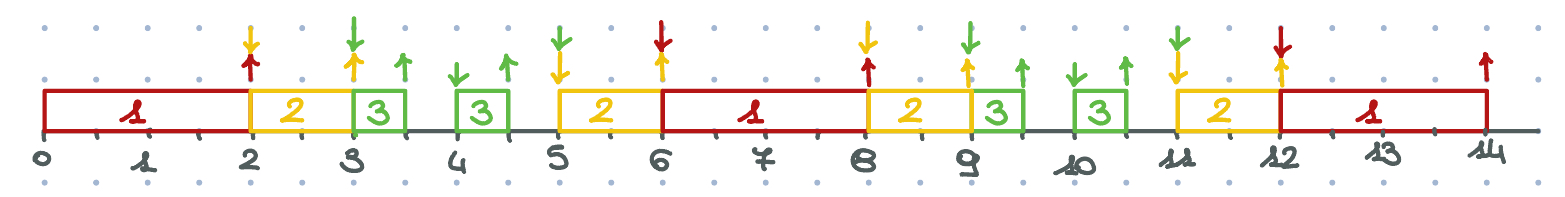
\includegraphics[width=14cm]{scheduling_without_custom.png}
\end{center}
As shown in the picture, at time 3.5s Task 3 is stopped and there's an empty space of 0.5 seconds, in which all the tasks are blocked, followed by the resumption of Task 3. This kind of behaviour is a huge loss of time since for 0.5 seconds all the tasks are blocked and the same TCB is extracted from the CPU, updated and then loaded again. To avoid this loss of time and power due to the context switching occurred, we want to modify the function in charge of inserting the task in the list of blocked tasks.\\
To do so we modify the function \texttt{vTaskDelay()} in the \texttt{task.c} file in order to perform a control before entering the task in the block list: if the block list contains already two of the three tasks then we verify if the delay time of the third task is minor or equal to the remaining delay time of the first element in the block list. If this condition is satisfied then the third task must not enter the block list and it should continue running until the first element of the block list gets ready.

\subsection{Benchmarks}
To do the benchmarks of this last explained implementation we can print on the screen the sequence of tasks and their starting and ending times in order to see if at critical times (like time 3.5s in this example) Task 3 is delayed or not.\\
We define the function \texttt{convertTicksToTime()} which has as parameters:
\begin{itemize}
    \item \texttt{TickType\_t ticks};
    \item \texttt{unsigned int *seconds};
    \item \texttt{unsigned int *milliseconds}:
\end{itemize}
and converts the ticks into seconds and milliseconds using the variable \texttt{TICKS\_PER\_SECOND} (equal to 1000).
After that, we need to timestamp for each task the tick of beginning and the tick of ending, convert them into seconds and milliseconds and then print them on the screen.\\
The final result is:
\begin{center}
  \includegraphics[width=13cm]{scheduling_with_custom1.png}
\end{center}
As shown in the picture the scheduling of the tasks is different: at time 3.5s Task 3 is no more delayed but it continues to work until time 5s, when the delay time of Task 3 is bigger than the remaining delay time of Task 2 and for this reason Task 3 is blocked for 0.5s and Task 2 is the first to start.\\
In this way we have optimized the usage of time by decreasing the number of context switches and by filling the empty spaces in those cases when all the tasks could be blocked contemporary.\\


\newpage 
\section{Bibliography}

\vspace{3ex}

Barry, R. \& The FreeRTOS Team. (2016). \href{https://www.freertos.org/Documentation/Mastering-the-FreeRTOS-Real-Time-Kernel.v1.0.pdf}{Mastering the FreeRTOS™ Real Time Kernel: A Hands-On Tutorial Guide}. Release Version 1.0. Real Time Engineers Ltd.\\

Noviello, C. (2022). Mastering STM32 - Second Edition. Release 2.0.1. Leanpub. \\

The FreeRTOS Team. (2017). \href{https://www.freertos.org/fr-content-src/uploads/2018/07/FreeRTOS_Reference_Manual_V10.0.0.pdf}{The FreeRTOS\texttrademark{} Reference Manual: API Functions and Configuration Options}. Version 10.0.0, issue 1. Amazon Web Services \\

\href{https://www.st.com/en/evaluation-tools/nucleo-f446re.html#documentation}{STM32 Nucleo-64 development board with STM32F446RE MCU Documentation}\\

\href{https://www.st.com/resource/en/user_manual/um1724-stm32-nucleo64-boards-mb1136-stmicroelectronics.pdf}{UM1724 User manual STM32 Nucleo-64 boards}\\

\href{https://www.keil.com/pack/doc/CMSIS/RTOS/html/functionOverview.html}{CMSIS-RTOS functions}\\


\section{Project contributions}

\begin{itemize}
    \item Jacopo Coniglio - exercise 1 for point 2; power point presentation;
    \item Francesca Coriale - exercise 2 for point 2; point 3 and 4 development; power point presentation;
    \item Sibilla Merlo - exercise 3 for point 2; report; power point presentation;
    \item Giulia Lydia Perini - point 1; report; power point presentation;
    \item Ankesh Porwal - exercise 0 point 2;
\end{itemize}

\end{document}
